\chapter*{Introduction}
%\chapter*{Preface}
%\addtocontents{toc}{Preface}
\addcontentsline{toc}{chapter}{Introduction}
\manualmark \markboth{}{Introduction}


%\section{Motivation}

%\todo{explain why DPPs are awesome}

%\section{Previous work}

%\section{Aim and outline of the dissertation}

%This dissertation emerged from the 



Before we introduce determinantal point processes (DPPs) mathematically we should give a short motivation for their study as well as an overview over the dissertation and its contributions. It is the goal to give a mostly self contained presentation to different approaches for the parameter estimation for DPPs that is accessible to any student familiar with the basic notions of linear algebra, analysis and probability theory. We prove most statements of this dissertation or give precise references if the statements are not assumed to be (mathematical) general knowledge.

\subsubsection*{Motivation}

Determinantal point processes are point processes, i.e. random subsets that exhibit a diversifying, repulsive behaviour in the sense that the subset is likely to obtain only elements that are different in some way. They arose first as the distribution of the eigenvalues of random matrices in \cite{mehta1960density} and later on in theoretical physics as the positions of Fermions like positively charged \(\alpha\)-particles that repell themselves (cf. \cite{benard1973detection}). Since then, they have appeared in the study of different random objects like non intersecting random walks and the descent positions in a random digit sequence (cf. \cite{johansson2004determinantal} and \cite{borodin2010adding}). The Wigner hypothesis states that the energy levels at which a neutron is scattered or reflected by heavy nuclei are distributed according to a DPP (cf. \cite{tao2010universality}). Furthermore, DPPs arise in number theory as it has been conjectured that the positions of the non trivial roots of the Riemannian zeta function are distributed according to a determinantal point process (cf. \cite{bourgade2013quantum}). Hence, DPPs are fundamental to different theories and are therefore highly interesting objects and a rich mathematical theory has been developed for them (cf. \cite{borodin2009determinantal}, \cite{hough2006determinantal}, \cite{lyons2003determinantal}).
In recent years DPPs have also been used to treat different real world phenomena and we will only present three of them shortly here.
\begin{enumerate}
\item \emph{Image search}: Assume we have given a set of \(10^6\) pictures that were returned by a search engine for a particular query. On the first page only a few, lets say \(20\) can be presented and in order to increase the probability that the user is satisfied with at least one picture it is favourable to include pictures that are not very similar in some notion. This can be modelled by a DPP since the goal is to select a diverse subset of pictures (cf. \cite{kulesza2011k}). % however one has to estimate 
\item \emph{Text summarisation:} DPPs have also been used successfully for extractive summarisation of news articles. The task of extractive summarisation is to select a subset of the sentences in order to obtain a reasonable summary of the text. The reason for the use of DPPs -- or any other diversifying point process -- is that similar sentences should not be selected for the summary since they would be quite repetitive then and hence only one of the sentences should be included in the summary (cf. \cite{kulesza2012learning1}). 
\item \emph{Pose selection:} One of the most impressive applications of DPPs has been found in the task of human pose extraction. The goal is -- given an image with an unknown amount of persons -- to schematically select their poses. A pose is associated with a quadrupel of rectangles which represent the head, torso and the two arms of a person. Since a picture consists of a finite number of pixels, the number of possible poses is also finite. It is possible to model how likely a certain pose is to be actually present in a given picture. If one would sample naively according to those probabilities one runs into the following problem: Similar poses usually have almost the same probability since they should describe the actual pose just about equally well. Hence, naive approaches are likely to select more than one of those poses for the same human.
\begin{figure}[h!]
	\centering
	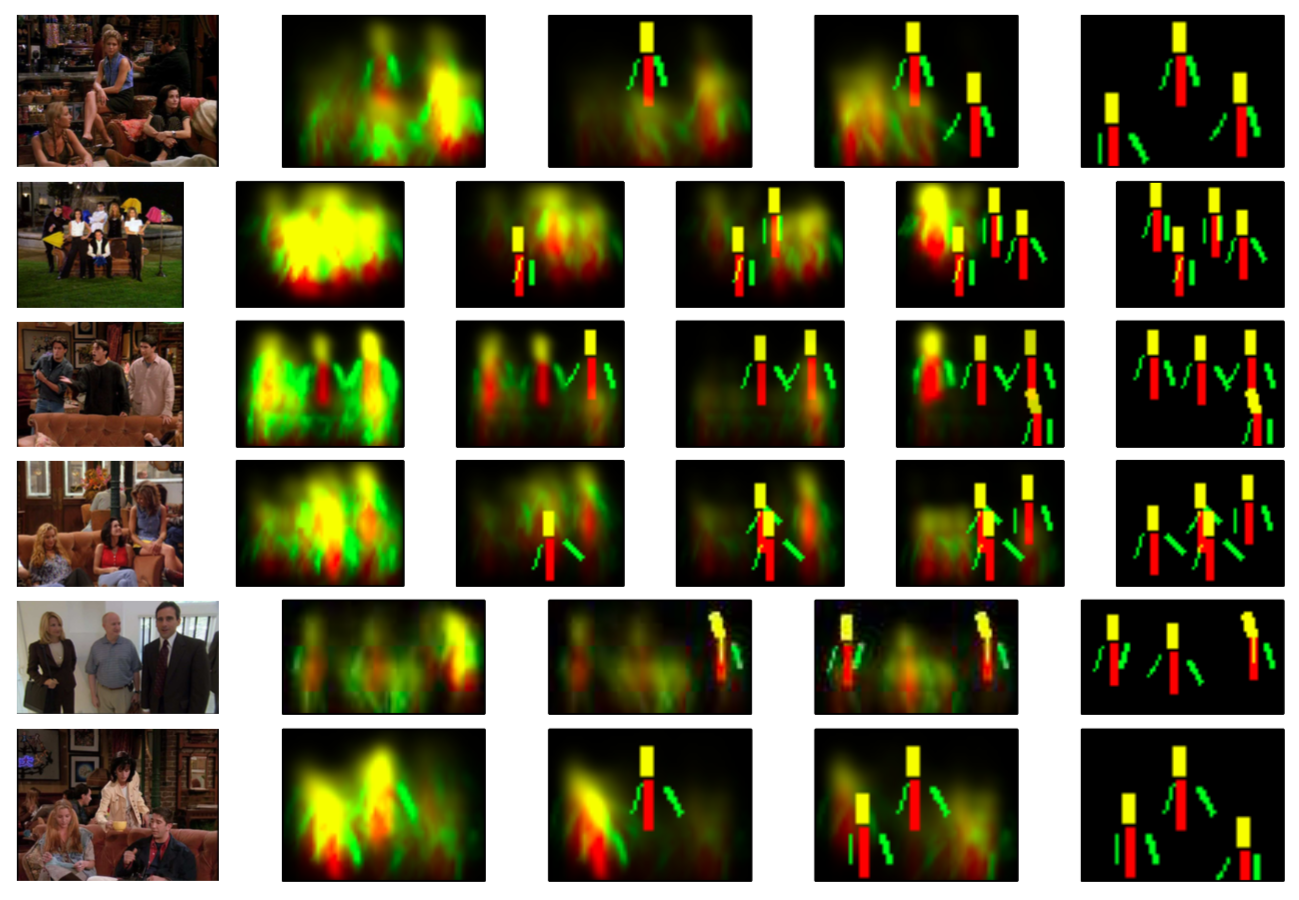
\includegraphics[width=0.99\textwidth]{figures/pose-estimation}
	\caption{The successive selection of poses in a picture using a DPP based on a the quality of the poses which is depicted in the second column. Original graphic due to \cite{kulesza2010structured}.}
	\label{fig:1}
\end{figure}
 This is where the repellent structure of a DPP can help to make it unlikely to select similar poses which leads to the effect that in most cases only one pose is selected for one person in the picture. This approach has successfully been taken in \cite{kulesza2010structured} and made it possible to perform the pose selection without the knowledge of the number of persons present in the picture.
\end{enumerate}

%In practice the procedure in those real world applications can be divided into two parts, the first one being the modelling of some properties of the phenomenon, the second one being the estimation of certain parameters. We will focus on the second part, since it is universal to a lot of real world applications and can be put into rigorous terms.
The procedure of the application of DPPs to those and further real world problems can roughly be divided into two parts. The first one consists of the selection of a suitable model for the given task and the second one of the estimation of 
%A crucial step in the application of DPPs to those and further real world problems is to estimate 
different parameters of the DPP which is the focus of this dissertation. % and hence it is of great interest how this can be done.

%\section{Historical remarks}
%\begin{enumerate}
%\item Theoretical work:
%\begin{enumerate}
%\item DPPs are point processes, i.e. random (locally finite) subsets that exhibit a diversifying, repulsive behaviour.
%\item They first arose as the positions of Fermions, for example positively charged \(\alpha\)-particles that repell themselves spatially or eigenvalues of random matrices.
%\item They continue to appear in
%\begin{enumerate}
%\item the study of many different random events like non intersection random walks and ...
%\item theoretical physics like the spectra of stars ...
%\item other areas of mathematics, for example the non trivial roots of the Riemmannian zeta function are conjectured to are distributed according to a DPP.
%\end{enumerate}
%\end{enumerate}
%\item In recent years DPPs have been used in the study of different real world phenomena including
%\begin{enumerate}
%\item Text summarisation
%\item Image search
%\item Pose estimation
% \item Applications to clustering
% \item Applications in computer vision (pose estimation special case)
%\end{enumerate}
%\item In practice the procedure in the procedure in those real world applications can be divided into two parts, the first one being the modelling of some properties of the phenomenon, the second one being the estimation of certain parameters. We will focus on the second part, since it is universal to a lot of real world applications and can be put into rigorous terms.
%\item All of applications include the estimation of the (some) parameters of the DPP and hence we will focus on this
%\end{enumerate}

\subsubsection{Outline of the thesis}
In the first chapter we introduce discrete determinantal point processes and present the fundamental concepts we will need. Further, we show that for a given marginal kernel a corresponding DPP exists and see how DPPs can be simulated and apply this to some toy examples. In the second chapter we will present two different ways to obtain an estimator for the marginal kernel or parametrisations of it. We will see that both strategies yield a consistent estimator and will discuss some of their benefits and hindrances. In the third chapter we will present the fundamentally different Bayesian approach to parameter estimation and apply it to the estimation of parameters of DPPs. In order to do this in practice we have to make use of Markov chain Monte Carlo (MCMC) methods and hence provide a minimalistic introduction to those. Finally we apply some of the presented estimation procedures to a toy example and will use this to investigate the effect of different regularisations. 
The appendix contains a collection of some statements used in the thesis, the R code that was used for the simulation of DPPs and also the parameter estimations that where performed.

\subsubsection{Contributions}
The dissertation is mainly based on the PhD thesis \cite{kulesza2012learning} and the research initiated by it, however, we provide a few novelties. We present a completely self contained presentation of the estimator of the marginal kernel that was first proposed in \cite{urschel2017learning} and give a different, arguably easier proof for the consistency of this estimator. Furthermore, we will provide proofs for the consistency of the maximum likelihood estimators for different parametric models of DPPs that could not be found in the literature so far.\footnote{At least to the best knowledge of the author.} In the last chapter we give a short introduction to MCMC methods including a collection of its mathematical foundations that is shorter -- and of course not as comprehensive -- than in most text books. We hope that the given toy examples help the understanding of DPPs and the influence on the different parameters to its properties. The provision of the code may be helpful to some readers, although it should be mentioned that the algorithms and their implementations were chosen for brevity and clarity and therefore may not be computationally optimal.


%\begin{enumerate}
%\item Outline:
%\begin{enumerate}
%\item Chapter I: Basics that we need to investigate the task of parameter estimation including the existence and simulation of DPPs and some toy examples.
%\item Chapter II: Presentation of two different point estimators including the proof of consistency of both.
%\item Chapter III: Discussion of a Bayesian framework for parameter estimation in general and for DPPs specifically including the benefits of this approach.
%\end{enumerate}
%\item Contributions:
%\begin{enumerate}
%\item Give a self contained presentation of the estimator for the marginal kernel that is presented in ... including a different, arguably easier proof of the consistency
%\item Show that the MLEs for different parameters exist with increasing probability and are in fact consistent.
%\item Give a short introduction into Bayesian parameter estimation and MCMC methods with a presentation of the mathematical foundations of those.
%\item Provide easy examples throughout the thesis including simulation and parameter estimations for those. The code for this is also included in the appendix.
%\end{enumerate}
%\item It is the aim to give a mostly self contained approach to the topic that is accessible to any student familiar with basic notions of linear algebra, analysis and probability theory. We proof almost everything we use in this dissertation or give precise references if the statements are not (mathematical) general knowledge.
%\end{enumerate}

%\automark % \markboth{}{Introduction}